% Options for packages loaded elsewhere
\PassOptionsToPackage{unicode}{hyperref}
\PassOptionsToPackage{hyphens}{url}
%
\documentclass[
]{article}
\usepackage{lmodern}
\usepackage{amsmath}
\usepackage{ifxetex,ifluatex}
\ifnum 0\ifxetex 1\fi\ifluatex 1\fi=0 % if pdftex
  \usepackage[T1]{fontenc}
  \usepackage[utf8]{inputenc}
  \usepackage{textcomp} % provide euro and other symbols
  \usepackage{amssymb}
\else % if luatex or xetex
  \usepackage{unicode-math}
  \defaultfontfeatures{Scale=MatchLowercase}
  \defaultfontfeatures[\rmfamily]{Ligatures=TeX,Scale=1}
\fi
% Use upquote if available, for straight quotes in verbatim environments
\IfFileExists{upquote.sty}{\usepackage{upquote}}{}
\IfFileExists{microtype.sty}{% use microtype if available
  \usepackage[]{microtype}
  \UseMicrotypeSet[protrusion]{basicmath} % disable protrusion for tt fonts
}{}
\makeatletter
\@ifundefined{KOMAClassName}{% if non-KOMA class
  \IfFileExists{parskip.sty}{%
    \usepackage{parskip}
  }{% else
    \setlength{\parindent}{0pt}
    \setlength{\parskip}{6pt plus 2pt minus 1pt}}
}{% if KOMA class
  \KOMAoptions{parskip=half}}
\makeatother
\usepackage{xcolor}
\IfFileExists{xurl.sty}{\usepackage{xurl}}{} % add URL line breaks if available
\IfFileExists{bookmark.sty}{\usepackage{bookmark}}{\usepackage{hyperref}}
\hypersetup{
  hidelinks,
  pdfcreator={LaTeX via pandoc}}
\urlstyle{same} % disable monospaced font for URLs
\usepackage{color}
\usepackage{fancyvrb}
\newcommand{\VerbBar}{|}
\newcommand{\VERB}{\Verb[commandchars=\\\{\}]}
\DefineVerbatimEnvironment{Highlighting}{Verbatim}{commandchars=\\\{\}}
% Add ',fontsize=\small' for more characters per line
\newenvironment{Shaded}{}{}
\newcommand{\AlertTok}[1]{\textcolor[rgb]{1.00,0.00,0.00}{\textbf{#1}}}
\newcommand{\AnnotationTok}[1]{\textcolor[rgb]{0.38,0.63,0.69}{\textbf{\textit{#1}}}}
\newcommand{\AttributeTok}[1]{\textcolor[rgb]{0.49,0.56,0.16}{#1}}
\newcommand{\BaseNTok}[1]{\textcolor[rgb]{0.25,0.63,0.44}{#1}}
\newcommand{\BuiltInTok}[1]{#1}
\newcommand{\CharTok}[1]{\textcolor[rgb]{0.25,0.44,0.63}{#1}}
\newcommand{\CommentTok}[1]{\textcolor[rgb]{0.38,0.63,0.69}{\textit{#1}}}
\newcommand{\CommentVarTok}[1]{\textcolor[rgb]{0.38,0.63,0.69}{\textbf{\textit{#1}}}}
\newcommand{\ConstantTok}[1]{\textcolor[rgb]{0.53,0.00,0.00}{#1}}
\newcommand{\ControlFlowTok}[1]{\textcolor[rgb]{0.00,0.44,0.13}{\textbf{#1}}}
\newcommand{\DataTypeTok}[1]{\textcolor[rgb]{0.56,0.13,0.00}{#1}}
\newcommand{\DecValTok}[1]{\textcolor[rgb]{0.25,0.63,0.44}{#1}}
\newcommand{\DocumentationTok}[1]{\textcolor[rgb]{0.73,0.13,0.13}{\textit{#1}}}
\newcommand{\ErrorTok}[1]{\textcolor[rgb]{1.00,0.00,0.00}{\textbf{#1}}}
\newcommand{\ExtensionTok}[1]{#1}
\newcommand{\FloatTok}[1]{\textcolor[rgb]{0.25,0.63,0.44}{#1}}
\newcommand{\FunctionTok}[1]{\textcolor[rgb]{0.02,0.16,0.49}{#1}}
\newcommand{\ImportTok}[1]{#1}
\newcommand{\InformationTok}[1]{\textcolor[rgb]{0.38,0.63,0.69}{\textbf{\textit{#1}}}}
\newcommand{\KeywordTok}[1]{\textcolor[rgb]{0.00,0.44,0.13}{\textbf{#1}}}
\newcommand{\NormalTok}[1]{#1}
\newcommand{\OperatorTok}[1]{\textcolor[rgb]{0.40,0.40,0.40}{#1}}
\newcommand{\OtherTok}[1]{\textcolor[rgb]{0.00,0.44,0.13}{#1}}
\newcommand{\PreprocessorTok}[1]{\textcolor[rgb]{0.74,0.48,0.00}{#1}}
\newcommand{\RegionMarkerTok}[1]{#1}
\newcommand{\SpecialCharTok}[1]{\textcolor[rgb]{0.25,0.44,0.63}{#1}}
\newcommand{\SpecialStringTok}[1]{\textcolor[rgb]{0.73,0.40,0.53}{#1}}
\newcommand{\StringTok}[1]{\textcolor[rgb]{0.25,0.44,0.63}{#1}}
\newcommand{\VariableTok}[1]{\textcolor[rgb]{0.10,0.09,0.49}{#1}}
\newcommand{\VerbatimStringTok}[1]{\textcolor[rgb]{0.25,0.44,0.63}{#1}}
\newcommand{\WarningTok}[1]{\textcolor[rgb]{0.38,0.63,0.69}{\textbf{\textit{#1}}}}
\usepackage{graphicx}
\makeatletter
\def\maxwidth{\ifdim\Gin@nat@width>\linewidth\linewidth\else\Gin@nat@width\fi}
\def\maxheight{\ifdim\Gin@nat@height>\textheight\textheight\else\Gin@nat@height\fi}
\makeatother
% Scale images if necessary, so that they will not overflow the page
% margins by default, and it is still possible to overwrite the defaults
% using explicit options in \includegraphics[width, height, ...]{}
\setkeys{Gin}{width=\maxwidth,height=\maxheight,keepaspectratio}
% Set default figure placement to htbp
\makeatletter
\def\fps@figure{htbp}
\makeatother
\setlength{\emergencystretch}{3em} % prevent overfull lines
\providecommand{\tightlist}{%
  \setlength{\itemsep}{0pt}\setlength{\parskip}{0pt}}
\setcounter{secnumdepth}{-\maxdimen} % remove section numbering
\ifluatex
  \usepackage{selnolig}  % disable illegal ligatures
\fi

\author{}
\date{}

\begin{document}

\hypertarget{header-n2}{%
\subsection{Task 2}\label{header-n2}}

\hypertarget{header-n3}{%
\subsubsection{1. Describe the Reuters-21578 corpus}\label{header-n3}}

Reuters-21578 is a test collection for text classification research that
is a multi-class, multi-label dataset. This dataset contains 90 classes,
7769 training files, and 3019 test files is a ModApte subdirectory of
the Reuters-21578 benchmark. The Reuters-21578 dataset was originally
collected and tagged by the Carnegie Group and Reuters in 1987 during
the development of the CONSTRUE text classification system, and later by
AT\&T Labs Research in September 1997. released in February, with David
D. Lewis as the lead publisher.

\hypertarget{header-n5}{%
\subsubsection{2. Describe how each document is represented in your
implementation.}\label{header-n5}}

\begin{Shaded}
\begin{Highlighting}[]
\SpecialCharTok{\textgreater{}} \FunctionTok{data}\NormalTok{(Reuters21578)}
\SpecialCharTok{\textgreater{}} \FunctionTok{class}\NormalTok{(Reuters21578)}
\NormalTok{[}\DecValTok{1}\NormalTok{] }\StringTok{"VCorpus"} \StringTok{"Corpus"} 
\SpecialCharTok{\textgreater{}} \FunctionTok{head}\NormalTok{(Reuters21578)}
\SpecialCharTok{\textless{}}\ErrorTok{\textless{}}\NormalTok{VCorpus}\SpecialCharTok{\textgreater{}}\ErrorTok{\textgreater{}}
\NormalTok{Metadata}\SpecialCharTok{:}\NormalTok{  corpus specific}\SpecialCharTok{:} \DecValTok{0}\NormalTok{, document }\FunctionTok{level}\NormalTok{ (indexed)}\SpecialCharTok{:} \DecValTok{0}
\NormalTok{Content}\SpecialCharTok{:}\NormalTok{  documents}\SpecialCharTok{:} \DecValTok{6}
\SpecialCharTok{\textgreater{}} \FunctionTok{summary}\NormalTok{(Reuters21578)}
\NormalTok{      Length Class             Mode}
\DecValTok{1}     \DecValTok{2}\NormalTok{      PlainTextDocument list}
\DecValTok{2}     \DecValTok{2}\NormalTok{      PlainTextDocument list}
\DecValTok{3}     \DecValTok{2}\NormalTok{      PlainTextDocument list}
\DecValTok{4}     \DecValTok{2}\NormalTok{      PlainTextDocument list}
\DecValTok{5}     \DecValTok{2}\NormalTok{      PlainTextDocument list}
\NormalTok{...}
\end{Highlighting}
\end{Shaded}

We import the Reuters-21578 as Vcorpus, which contains Metadata and
Content. The metadata attribute contains author, datetime stamp,
description, heading id, language, origin, lewissplit, cgisplit, oldid,
topics\_cat, places, people, orgs, exchanges. The content is the raw
data.

The data structure in the \texttt{tm} package that mainly manages
documents is called Corpus, which represents a collection of documents.
The corpus is divided into a dynamic corpus (Volatile Corpus) and a
static corpus (Permanent Corpus). A dynamic corpus will be stored in
memory as an R object and can be generated by either VCorpus() or
Corpus(). The dynamic corpus, on the other hand, is stored as an R
external file and can be generated using the PCorpus() function.

\hypertarget{header-n10}{%
\subsubsection{3. Describe the whole procedure on applying LDA to this
corpus to perform topic modeling.}\label{header-n10}}

\begin{enumerate}
\def\labelenumi{\arabic{enumi}.}
\item
  Import the dataset
\item
  Pre-processing the dataset, including transforming the content to
  lower case, striping whitespace, removing stopwords, punctuation and
  numbers, and steming document.
\item
  Calculate the BOW/TF-IDF document term matrix, \texttt{bowdtm} and
  \texttt{tfidfdtm}
\item
  Reducint the dimension with \texttt{tfidfdtm}
\item
  Calculate the word cloud with \texttt{bowdtm}
\item
  Apply LDA analysis.
\end{enumerate}

\hypertarget{header-n25}{%
\subsubsection{4. Describe the parameter setting that you use in the LDA
and explain their meanings.}\label{header-n25}}

\begin{Shaded}
\begin{Highlighting}[]
\NormalTok{result }\OtherTok{\textless{}{-}} \FunctionTok{LDA}\NormalTok{(bowdtm, k, }\AttributeTok{method=}\StringTok{"Gibbs"}\NormalTok{, }\AttributeTok{control=}\FunctionTok{list}\NormalTok{(}\AttributeTok{iter =} \DecValTok{25}\NormalTok{, }\AttributeTok{verbose =} \DecValTok{25}\NormalTok{, }\AttributeTok{alpha =} \FloatTok{0.1}\NormalTok{))}
\end{Highlighting}
\end{Shaded}

\texttt{bowdtm}: The document term matrix with BOW method.\\
\texttt{k}: number of topics\\
\texttt{method=Gibbs}: Applying Gibbs sampling\\
\texttt{control=list(iter\ =\ 25,\ verbose\ =\ 25,\ alpha\ =\ 0.1)}:
inference via 25 iterations.

\hypertarget{header-n29}{%
\subsubsection{5. Describe the output of your code and visualize the
obtained topics in appropriate ways.}\label{header-n29}}

Draw the word cloud from the TF-IDF document term matrix.\\
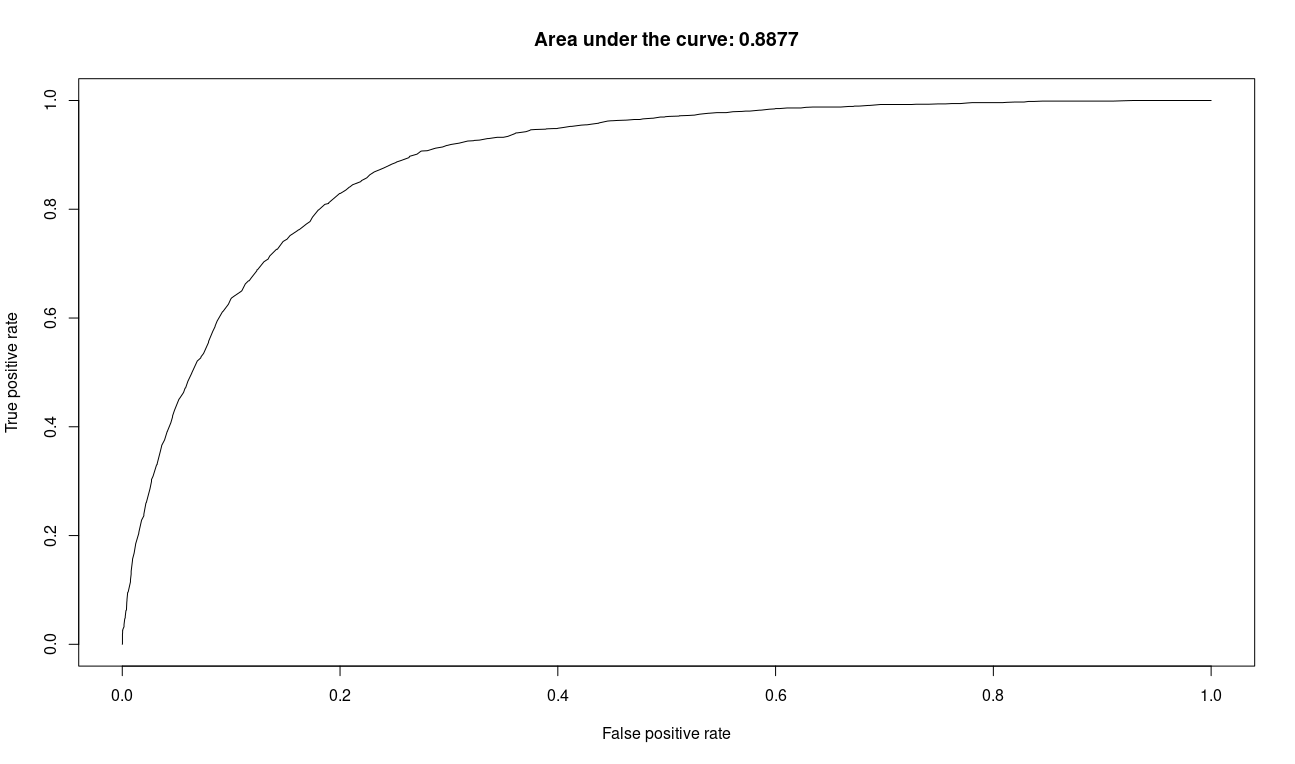
\includegraphics{/Users/maywzh/Workspace/ji_coursenotes/2020fall/CSCI946/assignment/ass2/task2/report/task2.1.png}\\
We can see that "cts", "mln" is the most frequent words.

\begin{Shaded}
\begin{Highlighting}[]
\SpecialCharTok{\textgreater{}}\NormalTok{ bowdtm }\OtherTok{\textless{}{-}}\NormalTok{ bowdtm[slam}\SpecialCharTok{::}\FunctionTok{row\_sums}\NormalTok{(bowdtm) }\SpecialCharTok{\textgreater{}} \DecValTok{0}\NormalTok{, ]}
\SpecialCharTok{\textgreater{}}\NormalTok{ k }\OtherTok{\textless{}{-}} \DecValTok{20}
\SpecialCharTok{\textgreater{}}\NormalTok{ result }\OtherTok{\textless{}{-}} \FunctionTok{LDA}\NormalTok{(bowdtm, k, }\AttributeTok{method=}\StringTok{"Gibbs"}\NormalTok{, }\AttributeTok{control=}\FunctionTok{list}\NormalTok{(}\AttributeTok{iter =} \DecValTok{25}\NormalTok{, }\AttributeTok{verbose =} \DecValTok{25}\NormalTok{, }\AttributeTok{alpha =} \FloatTok{0.1}\NormalTok{))}
\NormalTok{K }\OtherTok{=} \DecValTok{20}\NormalTok{; V }\OtherTok{=} \DecValTok{32697}\NormalTok{; M }\OtherTok{=} \DecValTok{19042}
\NormalTok{Sampling }\DecValTok{25}\NormalTok{ iterations}\SpecialCharTok{!}
\NormalTok{Iteration }\DecValTok{25}\NormalTok{ ...}
\NormalTok{Gibbs sampling completed}\SpecialCharTok{!}
\ErrorTok{\textgreater{}}\NormalTok{ result}
\NormalTok{A LDA\_Gibbs topic model with }\DecValTok{20}\NormalTok{ topics.}
\SpecialCharTok{\textgreater{}} \FunctionTok{terms}\NormalTok{(result, }\DecValTok{10}\NormalTok{)}
\NormalTok{      Topic }\DecValTok{1}\NormalTok{   Topic }\DecValTok{2}\NormalTok{   Topic }\DecValTok{3}\NormalTok{   Topic }\DecValTok{4}\NormalTok{    Topic }\DecValTok{5}\NormalTok{   Topic }\DecValTok{6}\NormalTok{   Topic }\DecValTok{7}\NormalTok{   Topic }\DecValTok{8}\NormalTok{      Topic }\DecValTok{9}\NormalTok{    Topic }\DecValTok{10}\NormalTok{  Topic }\DecValTok{11}\NormalTok{  Topic }\DecValTok{12}\NormalTok{  Topic }\DecValTok{13}\NormalTok{  Topic }\DecValTok{14}\NormalTok{ Topic }\DecValTok{15} 
\NormalTok{ [}\DecValTok{1}\NormalTok{,] }\StringTok{"said"}    \StringTok{"said"}    \StringTok{"said"}    \StringTok{"said"}     \StringTok{"dlrs"}    \StringTok{"billion"} \StringTok{"said"}    \StringTok{"tonn"}       \StringTok{"bank"}     \StringTok{"said"}    \StringTok{"said"}    \StringTok{"oil"}     \StringTok{"said"}    \StringTok{"pct"}    \StringTok{"said"}   
\NormalTok{ [}\DecValTok{2}\NormalTok{,] }\StringTok{"govern"}  \StringTok{"will"}    \StringTok{"trade"}   \StringTok{"trade"}    \StringTok{"mln"}     \StringTok{"bank"}    \StringTok{"market"}  \StringTok{"said"}       \StringTok{"said"}     \StringTok{"share"}   \StringTok{"reuter"}  \StringTok{"said"}    \StringTok{"export"}  \StringTok{"will"}   \StringTok{"share"}  
\NormalTok{ [}\DecValTok{3}\NormalTok{,] }\StringTok{"econom"}  \StringTok{"compani"} \StringTok{"japan"}   \StringTok{"reuter"}   \StringTok{"said"}    \StringTok{"pct"}     \StringTok{"rate"}    \StringTok{"mln"}        \StringTok{"debt"}     \StringTok{"compani"} \StringTok{"mine"}    \StringTok{"price"}   \StringTok{"will"}    \StringTok{"issu"}   \StringTok{"stock"}  
\NormalTok{ [}\DecValTok{4}\NormalTok{,] }\StringTok{"japan"}   \StringTok{"new"}     \StringTok{"offici"}  \StringTok{"futur"}    \StringTok{"year"}    \StringTok{"franc"}   \StringTok{"dollar"}  \StringTok{"wheat"}      \StringTok{"loan"}     \StringTok{"stock"}   \StringTok{"gold"}    \StringTok{"gas"}     \StringTok{"produc"}  \StringTok{"said"}   \StringTok{"compani"}
\NormalTok{ [}\DecValTok{5}\NormalTok{,] }\StringTok{"offici"}  \StringTok{"reuter"}  \StringTok{"state"}   \StringTok{"price"}    \StringTok{"quarter"} \StringTok{"said"}    \StringTok{"bank"}    \StringTok{"export"}     \StringTok{"billion"}  \StringTok{"reuter"}  \StringTok{"will"}    \StringTok{"barrel"}  \StringTok{"price"}   \StringTok{"mln"}    \StringTok{"inc"}    
\NormalTok{ [}\DecValTok{6}\NormalTok{,] }\StringTok{"minist"}  \StringTok{"car"}     \StringTok{"import"}  \StringTok{"pct"}      \StringTok{"compani"} \StringTok{"year"}    \StringTok{"trade"}   \StringTok{"reuter"}     \StringTok{"dlrs"}     \StringTok{"court"}   \StringTok{"compani"} \StringTok{"product"} \StringTok{"coffe"}   \StringTok{"bond"}   \StringTok{"dlrs"}   
\NormalTok{ [}\DecValTok{7}\NormalTok{,] }\StringTok{"year"}    \StringTok{"trade"}   \StringTok{"japanes"} \StringTok{"new"}      \StringTok{"sale"}    \StringTok{"mln"}     \StringTok{"analyst"} \StringTok{"agricultur"} \StringTok{"will"}     \StringTok{"offer"}   \StringTok{"ton"}     \StringTok{"mln"}     \StringTok{"reuter"}  \StringTok{"dlrs"}   \StringTok{"offer"}  
\NormalTok{ [}\DecValTok{8}\NormalTok{,] }\StringTok{"will"}    \StringTok{"motor"}   \StringTok{"unit"}    \StringTok{"cent"}     \StringTok{"earn"}    \StringTok{"reuter"}  \StringTok{"currenc"} \StringTok{"year"}       \StringTok{"interest"} \StringTok{"file"}    \StringTok{"oper"}    \StringTok{"compani"} \StringTok{"meet"}    \StringTok{"rate"}   \StringTok{"will"}   
\NormalTok{ [}\DecValTok{9}\NormalTok{,] }\StringTok{"west"}    \StringTok{"exchang"} \StringTok{"will"}    \StringTok{"tonn"}     \StringTok{"share"}   \StringTok{"foreign"} \StringTok{"dealer"}  \StringTok{"grain"}      \StringTok{"countri"}  \StringTok{"board"}   \StringTok{"ounc"}    \StringTok{"dlrs"}    \StringTok{"countri"} \StringTok{"reuter"} \StringTok{"reuter"} 
\NormalTok{[}\DecValTok{10}\NormalTok{,] }\StringTok{"japanes"} \StringTok{"market"}  \StringTok{"reuter"}  \StringTok{"contract"} \StringTok{"report"}  \StringTok{"mark"}    \StringTok{"exchang"} \StringTok{"crop"}       \StringTok{"new"}      \StringTok{"inc"}     \StringTok{"power"}   \StringTok{"will"}    \StringTok{"quota"}   \StringTok{"manag"}  \StringTok{"common"} 
\NormalTok{      Topic }\DecValTok{16}\NormalTok{  Topic }\DecValTok{17}\NormalTok{  Topic }\DecValTok{18}\NormalTok{  Topic }\DecValTok{19}\NormalTok{ Topic }\DecValTok{20}  
\NormalTok{ [}\DecValTok{1}\NormalTok{,] }\StringTok{"said"}    \StringTok{"said"}    \StringTok{"said"}    \StringTok{"mln"}    \StringTok{"pct"}     
\NormalTok{ [}\DecValTok{2}\NormalTok{,] }\StringTok{"tax"}     \StringTok{"compani"} \StringTok{"compani"} \StringTok{"cts"}    \StringTok{"year"}    
\NormalTok{ [}\DecValTok{3}\NormalTok{,] }\StringTok{"billion"} \StringTok{"dlrs"}    \StringTok{"will"}    \StringTok{"net"}    \StringTok{"said"}    
\NormalTok{ [}\DecValTok{4}\NormalTok{,] }\StringTok{"budget"}  \StringTok{"reuter"}  \StringTok{"reuter"}  \StringTok{"loss"}   \StringTok{"billion"} 
\NormalTok{ [}\DecValTok{5}\NormalTok{,] }\StringTok{"bill"}    \StringTok{"share"}   \StringTok{"inc"}     \StringTok{"dlrs"}   \StringTok{"februari"}
\NormalTok{ [}\DecValTok{6}\NormalTok{,] }\StringTok{"stg"}     \StringTok{"mln"}     \StringTok{"corp"}    \StringTok{"shr"}    \StringTok{"januari"} 
\NormalTok{ [}\DecValTok{7}\NormalTok{,] }\StringTok{"hous"}    \StringTok{"corp"}    \StringTok{"system"}  \StringTok{"reuter"} \StringTok{"rose"}    
\NormalTok{ [}\DecValTok{8}\NormalTok{,] }\StringTok{"dlrs"}    \StringTok{"inc"}     \StringTok{"new"}     \StringTok{"profit"} \StringTok{"rise"}    
\NormalTok{ [}\DecValTok{9}\NormalTok{,] }\StringTok{"reuter"}  \StringTok{"group"}   \StringTok{"servic"}  \StringTok{"rev"}    \StringTok{"last"}    
\NormalTok{[}\DecValTok{10}\NormalTok{,] }\StringTok{"bank"}    \StringTok{"will"}    \StringTok{"comput"}  \StringTok{"oper"}   \StringTok{"month"}  
\end{Highlighting}
\end{Shaded}

We should remove empty rows in \texttt{bowdtm} and set number of topics
to 20. Then we can compute the LDA model, inferencing via 25 iterations
of Gibbs sampling.

We can see the 10 most likely terms within the term probabilities beta
of the inferred topics.

We took eight sample documents:

\begin{Shaded}
\begin{Highlighting}[]
\NormalTok{examples }\OtherTok{\textless{}{-}} \FunctionTok{c}\NormalTok{(}\DecValTok{2}\NormalTok{, }\DecValTok{100}\NormalTok{, }\DecValTok{200}\NormalTok{, }\DecValTok{400}\NormalTok{, }\DecValTok{800}\NormalTok{, }\DecValTok{1000}\NormalTok{, }\DecValTok{1200}\NormalTok{, }\DecValTok{1400}\NormalTok{)}
\FunctionTok{lapply}\NormalTok{(pre\_process\_reuters[examples], as.character)}

\NormalTok{theta }\OtherTok{\textless{}{-}}\NormalTok{ tmposterior}\SpecialCharTok{$}\NormalTok{topics}
\NormalTok{N }\OtherTok{\textless{}{-}} \FunctionTok{length}\NormalTok{(examples)}

\NormalTok{tpExamples }\OtherTok{\textless{}{-}}\NormalTok{ theta[examples,]}
\FunctionTok{colnames}\NormalTok{(tpExamples) }\OtherTok{\textless{}{-}}\NormalTok{ nameOfTopics}
\NormalTok{vizDataFrame }\OtherTok{\textless{}{-}} \FunctionTok{melt}\NormalTok{(}\FunctionTok{cbind}\NormalTok{(}\FunctionTok{data.frame}\NormalTok{(tpExamples), }\AttributeTok{document =} \FunctionTok{factor}\NormalTok{(}\DecValTok{1}\SpecialCharTok{:}\NormalTok{N)), }\AttributeTok{variable.name =} \StringTok{"topic"}\NormalTok{, }\AttributeTok{id.vars =} \StringTok{"document"}\NormalTok{)  }
\NormalTok{vizDataFrame}
\end{Highlighting}
\end{Shaded}

and get topic proportions form example documents.

\begin{figure}
\centering
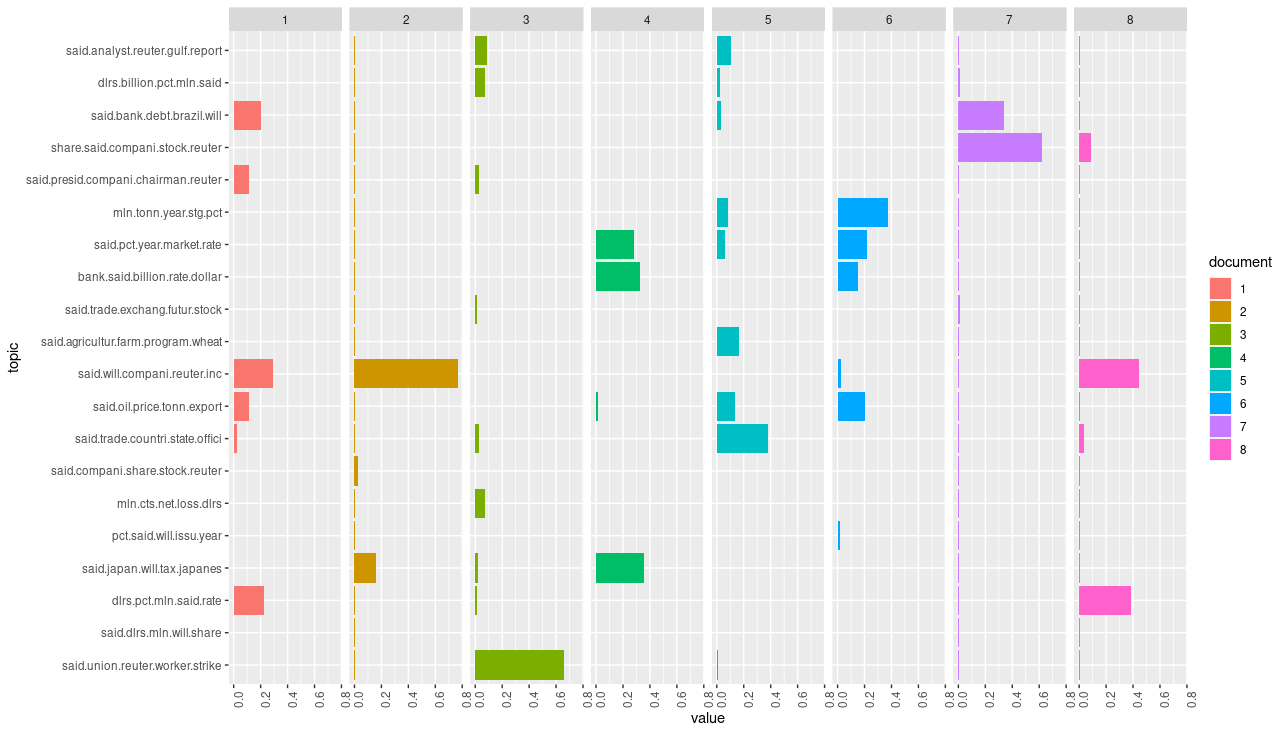
\includegraphics{/Users/maywzh/Workspace/ji_coursenotes/2020fall/CSCI946/assignment/ass2/task2/report/task2.2.png}
\caption{}
\end{figure}
\hypertarget{header-n39}{%
\subsubsection{6. Attach your code to the ZIP file.}\label{header-n39}}

\end{document}
